\documentclass[12p]{article}

\usepackage[english]{babel}
\usepackage[utf8x]{inputenc}
\usepackage[colorinlistoftodos]{todonotes}
\usepackage{fancyhdr} %Package to configure headings and footer
\usepackage{lastpage} %Needed to display last page (total amount of pages)
\usepackage{listings}

% pagelayout
\usepackage[
top    = 2.75cm,
bottom = 2.00cm,
left   = 2.50cm,
right  = 2.00cm]{geometry}
\setcounter{secnumdepth}{4}

% header
\pagestyle{fancy}
\fancyhead[L]{\today}
\fancyhead[R]{Load Balancing - Gliederung}

%footer
\fancyfoot[L]{Haidn, Schrack}
\fancyfoot[C]{5A HIT}
\fancyfoot[R]{Seite \thepage/\pageref{LastPage}}

%title page
\author{Martin Haidn, Nikolaus Schrack}
\title{Load Balancing - Structure\\SYT - 5A HIT}
\date{\today}

%Glossary
\usepackage{glossaries}
\makeglossaries
\newglossaryentry{mac}{name=MAC, description={Media Access Controll}}

\begin{document}
	\maketitle
	
	\newpage
	\tableofcontents
	
	\newpage
	\section{Instruction}
	
	The concept of Load Balancing is not new in the server and network space. There are different types of Load Balancing. A Router, for example, distributes the traffic across multiple paths to the same destination. A Server Load Balancer, on the other hand, distributes traffic among server resources rather then network resources. \cite{lb_SFC}  \\ \\
	Typically it is used for balancing traffic over multiple servers and acting as one web front-end. The user usually doesn't know about the existence of multiple backend servers because it seems as there is only one server. The processing load is shared across many nodes, rather than just to a single server. Thus the performance during times of high activity increases.
	\cite{liquidweb}
	
	
	\subsection{The Need and Goals for Load Balancing}
	%This section should describe what's the aim of using load distribution and why or %respectively where it's needed.
	 %It is better to use multiple components with load balancing to increace the reliability throguh redundancy. 	 
	
	
	The main goal of Load Balancing is to distribute workload across resources. It is suppose to optimize the traffic, maximaize throughput, minimize response time and try not to overload any single resources. \\\\
	Since the Internet and Intranet have gotten so important for businesses, Load Balancing has become a very essential component for networks and servers. If the network goes down or works poorly, it can critically damage a business. Especially for companies with e-commerce a long respond time or in the worst case an outage would leave frustrated customers and huge money loss. For other companies loosing access to email would have devastating impact on their business.  \cite{lb_SFC} \\\\
	The problem of scaling computer capacity is also important. In the old days, if a server wasn't good enough to run an application they simply bought a more powerful.  Nowadays the Load Balancing systems work with multiple servers. If the traffic becomes more and more, one should just be able to hang another server into the balancing and it should work.\cite{lb_SFC} \\\\
	There are two main reasons for Load Balancing: 
	\begin{enumerate}
		\item Limiting your points of failure
		\item Load Distribution
	\end{enumerate} 
	\textbf{Limiting your points of failure} is essential for every IT Department. The uptime increases by the limitation of available points of failure. "If you load balance between two or more identical nodes, in the event that one of the nodes in your cluster experiences any kind of hardware or software failure the traffic can be redistributed to the other nodes keeping your site up." \cite{liquidweb} Those identical servers can independently handle the traffic. If there is a failure in one of them the site still runs.
	\\\\
	\textbf{Load Distribution} 
	A single server configuration can only hold a certain amount of traffic, even the most robust, high-end server. But at the traffic peaks of the application it still needs to work just fine. As website grows popularity, multiple servers with Load Balancing are necessary. \cite{liquidweb}
		
	\subsection{Use Cases and Examples}
	This section should pick up the significant points from the "Needs and Goals" and bring them in a relation with specific, real examples.
	\subsection{Applications}
	%An overview about the common used applications %for load distribution.
	With the rise of the Internet, the network becomes very important. "As the Internet connects the world and the Intranet becomes the operational backbone for businesses, the IT infrastructure can be thought of as two types of equipment: computer that function as a client and/or a server, and switches/routers that connect the computers"\cite{lb_SFC} \\
	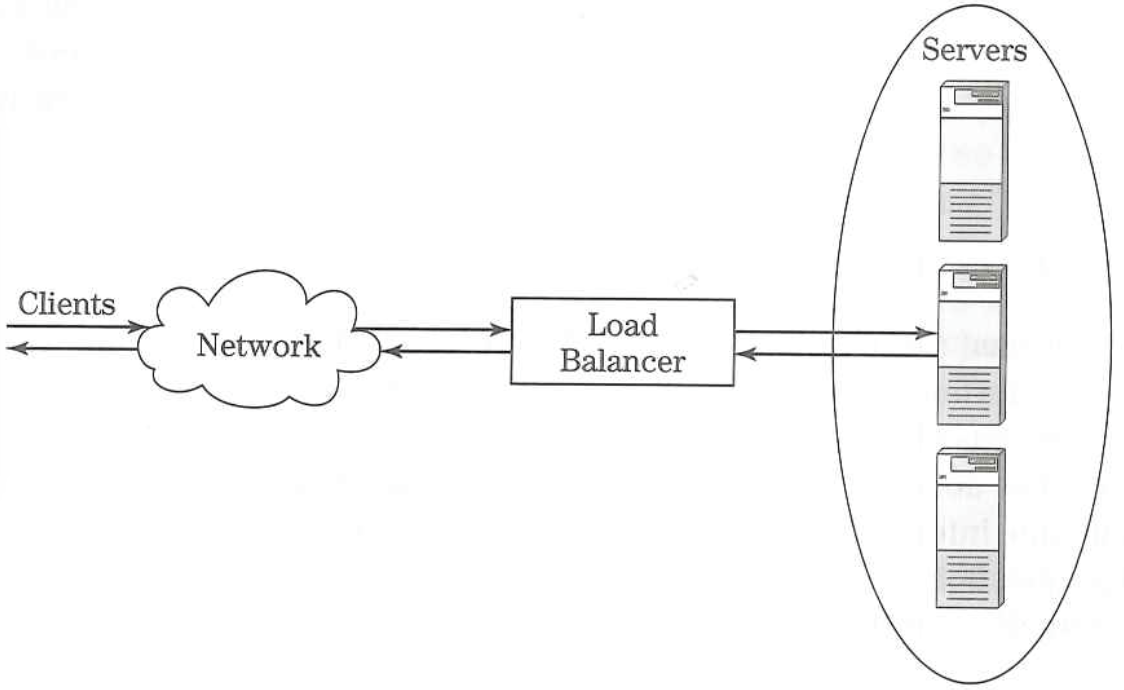
\includegraphics[width=\textwidth]{basic}\cite{lb_SFC} \\\\
	The grafic shows that the Load Balancer is the connection between the clients and the servers. The Load Blancer understands many higher-layer protocols, so they can communicate with servers intelligently. They also understand networking protocols, so they can work with the network effectively.\\\\
	Load Balancer have four big applications
	\begin{enumerate}
		\item Server load balancing
		\item Global load balancing
		\item Firewall load balancing
		\item Transparent cache switching
	\end{enumerate} 
	Server load balancing deals with multiple servers to scale beyond the capacity of one server and to handle a server failure. Global load balancing directs users to different data centers consisting of server farms so they can provide quicker response and handle a data center failure. The Firewall Load balancing can distribute load between multiple firewalls to again, handle a failure of one of them. Transparent cache switching directs traffic to caches to minimize the response time. \\ \\
	There are three main forms of products for load balancing. 
	\begin{enumerate}
		\item Software load-balancing
		\item Appliances
		\item Switches
	\end{enumerate}
	\textbf{Software load balancing} are products that run on load balancing servers. They have algorithms to coordinate the traffic among them. For example Apache Module mod\_proxy is a popular tool. Nginx would be another tool that allows software load balancing. They are mostly for free which is great if one runs on a low budget.  \\\\ % TODO: kann man noch weiter ausfuehren
	\textbf{Appliances} are a all-in-one product that include necessary hardware and software to do web switching. It may has some special operating system and custom hardware. For example Cisco has hardware appliances that handle load balancing for you. \\\\ % TODO: More examples ...	
	\textbf{Switches} have to their traditional functionality in OSI Layer 2/3, are also able to do load balancing on Layer 4-7. Mostly though, they a significant amount of work done by software. For example Zen Load Balancer  and Cisco as well have switches  appliances that handle load balancing for you.
	\newpage
	\section{Basic Concepts}
	\subsection{Networking Fundamentals}
	The OSI model contains seven layers and every single one provides it's own functionality and data.\\
	If we take a closer look on the deeper layers like data link and network, which is representative for layer two and three, we can see that their header information contains IP and MAC addresses. These addresses can be used to decide where a package has to be send when it's revived by a switch.\\
	This basic concept of routing packages builds the fundament for load balancing. It's about making a decision if, and where the data has to go. \cite{lb_SFC}
	\subsection{Higher Layered Distribution}
	Description how load distribution works on OSI-Layers six and seven.
	\subsection{Load-Distribution Methods}
	Summary of common load distribution Methods, their benefits and disadvantages.
	
	\newpage
	\section{Advanced Concepts}
	\subsection{Session Persistence}
	A way of load distribution where the balancer has to store the whole session information during the time of an application transaction is called Session Persistence. In addition to the right client address the balancer also has to know about the correct server, the request got forwarded to. This concept is mostly used on web services where the server has to respond with user specific content or data.\\
	For Example you can imagine an on-line book store which provides a shopping cart function that keeps your articles during your stay. If the load balancer would not store the session information during your purchase the selected article would probably get lost or in the worst case inverted with the goods of another user.\\
	The way to get the information which is needed is broadly based onto two sources:\\
	\\
	\textbf{TCP SYN Packet}\\
	TCP SYN is the first request the clients sends to the server if he wants to establish a new connection.\\
	It contains the source IP address and port to identify the user and also the destination Ip and port to identify the server.\\
	\\
	\textbf{Application Request}
	If the user calls an application or a method on the server the request has to be defined in the send packages.\\
	This information is used by the balancer to forward the request to the right providing server.
	\subsection{URL Switching}
	The flexibility of layer seven load balancing and the included url switching.
	\subsection{Network-Address Translation}
	Fast Layer 4 load balancing and the appliance as default gateway.
	
	\newpage
	\section{Scheduling Algorithms}
	\subsection{Weighted Balance}
	Ways to guarantee a weighted balance in busy systems.
	\subsection{Priority}
	The meaning of priorities concerning the process of load balancing and how to route traffic to a preferred link, as long it's available.
	\subsection{Overflow}
	How to prevent traffic flow from slowing down when the connection runs out of available bandwidth.
	\subsection{Persistance}
	Eliminate session termination issue for HTTPS, E-banking, and other secure websites.
	\subsection{Round-Robin}
	A closer explanation to the scheduling procedure "Round Robin"
	
	\newpage
	\section{Caches}
	\subsection{Definition}
	Define what a cache is for when we talk about load balancing.
	\subsection{Types}
	The different types of caches and their usage as well as benefits and disadvantages.
	\subsection{Deployment}
	Examples and explanation how to deploy load distribution using caches.
	
	\newpage
	\section{Problems}
	\subsection{Mega Proxy Session}
	Problems triggered through the use of Mega Proxys on the client site.
	
	\newpage
	\printglossaries
	
	\newpage
	\bibliographystyle{plain}
	\bibliography{Loadbalancing_Haidn_Schrack.bib}
	
	\newpage
	\section{Sources}
	\todo{Please note that this is just an overview about our collected references so far, to find them in the TU-Library. We'll add our last visits during this elaberation.}
	Titel:    Load balancing servers, firewalls, and caches : [timely, practical, reliable]\\
	Autor:    Chandra Kopparapu\\
	Jahr:    2002\\
	ISBN:    ISBN 0-471-41550-2\\
	TUWS:    DAT:964, DAT:224\\
	\\
	Titel:    Dynamic load balancing : an overview\\
	Autor:    Arnold R. Krommer ; Christoph W. Ueberhuber\\
	Jahr:    1992\\
	ISBN:     -\\
	TUWS:    DAT:351\\
	\\
	Titel:    Dynamischer Lastausgleich in Parallelrechnersystemen : genetische Algorithmen und eine spezielle Rechnerstruktur\\
	Autor:    Michael Witt\\
	Jahr:    1997\\
	ISBN:    -\\
	TUWS:    -\\
	\\
	Titel:    Optimal load balancing in distributed computer systems\\
	Autor:    Hisao Kameda\\
	Jahr:    1997\\
	ISBN:    ISBN 3-540-76130-6\\
	TUWS:     -\\
	\\
	\\
	Titel:     Server Load Balancing\\
	Autor:     Tony Bourke\\
	Jahr:     August 2001\\
	0-596-00050-2, Order Number: 0502\\
	200 pages, 34.95 USD\\
	Link: http://oreilly.com/catalog/serverload/chapter/ch07.html\\
	\\
	\\
	Onlinequellen:\\
	\\
	Name:    Optimal Load Balancing in Distributed Computer Systems\\
	Link:    http://bookzz.org/book/2092081/f777c1\\
	\\
	Name:    Spectral Methods for Efficient Load Balancing Strategies\\
	Link:    http://cs.emis.de/LNI/Dissertation/Dissertation3/GI-Dissertations.03-3.pdf\\
	\\
	Name:    Lastverteilung auf dem Konzept des virtuellen Servers\\
	Link:    http://www.nm.ifi.lmu.de/pub/Fopras/fikr02/PDF-Version/fikr02.pdf\\
	\\
	Name: Dynamic Load Balancing and Scheduling\\
	Link: http://www2.cs.uni-paderborn.de/cs/ag-monien/RESEARCH/LOADBAL/\\
	\\
	
\end{document}